\documentclass[UTF8]{ctexart}
\usepackage{amsmath}
\usepackage{diagbox}
\usepackage{textcomp}
\usepackage{graphicx}
\usepackage{float}
\usepackage{caption}
\usepackage{adjustbox}
\usepackage{subfigure}
\usepackage{geometry}
\usepackage{pifont}
\usepackage{gensymb}
\usepackage{bm}
\begin{document}
\renewcommand{\thefootnote}{\fnsymbol{footnote}}
\newgeometry{left=2cm,bottom=4cm,right=2cm}
\linespread{1.4}
\title{\vspace{-5em}\heiti电磁感应实验报告\vspace{-2.5em}}
\date{}
\maketitle
\begin{center}
{\fangsong 徐浩博\quad 软件02\quad2020010108}
\end{center}

\subsubsection*{摘要}
{\kaishu\normalsize  本实验旨在通过自感、互感、电磁感应等实验现象的观察,测量出电阻、感抗、互感、铝芯涡流损耗等一系列数据,使我掌握了电路连接、万用表使用等的知识,并对自感、互感、电磁感应等相关知识有了更深的理解. 同时,我还通过相关计算进一步巩固了实验误差的分析、直线拟合、利用数据作图和分析等相关知识.}
\subsubsection*{关键词:电磁感应\quad 自感\quad  互感\quad  耦合系数\quad 等效感抗 \quad 反射感抗 \quad  涡流损耗\vspace{1.5em}}

\[\frac{U_Q}{Q}=\frac{U_\xi}{\xi}\]
\section{实验仪器}
本实验用到的主要仪器有:\par
1) 正弦波发生器及BNC转香蕉插头\par
2) 电阻板、面包板、连接线\par
3) 两个缠绕紧密的耦合线圈和铝芯\par
4) 数字万用表

\section{实验原理及实验数据}

\subsection*{第一部分:测量无芯线圈和铝芯线圈的电阻和电感}
\subsubsection*{a)测量无芯线圈1的电阻和电感}
\begin{figure}[H]\begin{center}
    \includegraphics*[scale = 0.3]{1.png}
\end{center}\end{figure}
\vspace{-2em}
对于一个RL暂态电路,假设电阻电感分别为R和L,则欧姆定律可以写作:

\begin{equation}
    \tilde{U}=\tilde{I}(i\omega L+R)
\end{equation}
若以电流相位为0,则电压相位如下图所示:
\begin{figure}[H]\begin{center}
    \includegraphics*[scale = 0.25]{2.png}
\end{center}\end{figure}
\vspace{-2em}
可写作:
\begin{equation}
    \tan\theta=\frac{\omega L}{R}=\frac{X}{R}
\end{equation}
考虑到U和I有效值正比于$\tilde{U}$和$\tilde{I}$振幅,且比率系数相等,故对(1)式取模可以得到:
\begin{equation}
    V=I\sqrt{\omega^2 L^2+R^2}=I\sqrt{X^2+R^2}
\end{equation}
其中V, I是电压、电流有效值,$X=\omega L$为感抗. 联立(2)(3)式有:
\begin{equation}
    V\cos\theta=IR
\end{equation}
那么对于下面电路,我们可以分别写出基尔霍夫定律和欧姆定律:
\begin{figure}[H]\begin{center}
    \includegraphics*[scale = 0.4]{3.png}
\end{center}\end{figure}
\vspace{-2em}
\begin{equation} 
    \begin{aligned}
        &\tilde{U_A}=\tilde{U}+\tilde{U_{R'}}\\
    \end{aligned}
\end{equation}
画出复数三角形如下图:
\begin{figure}[H]\begin{center}
    \includegraphics*[scale = 0.4]{4.png}
\end{center}\end{figure}
\vspace{-2em}
于是由余弦定理:
\begin{equation}
    |\tilde{U_A}|^2=|\tilde{U_{R'}}|^2+|\tilde{U}|^2+2|\tilde{U_{R'}}||\tilde{U}|\cos\theta
\end{equation}
写成有效值形式为:
\begin{equation}
    {V_A}^2={V_{R'}}^2+{V}^2+2V_{R'}{V}\cos\theta
\end{equation}
对于R',列出欧姆定律:
\begin{equation}
    V_{R'}=IR'
\end{equation}
联立(4)(7)(8)式可以得到线圈电阻值:
\begin{equation}
    R=\frac{R'}{2}(\frac{V_A^2-V^2}{V_{R'}^2}-1)
\end{equation}
联立(3)(8)式可以得到线圈电感值:
\begin{equation}
    L=\frac{1}{\omega}\sqrt{\frac{V^2}{V_{R'}^2}R'^2-R^2}
    =\frac{1}{2\pi f}\sqrt{\frac{V^2}{V_{R'}^2}R'^2-R^2}
\end{equation}
据(9)(10)式,我们可以通过给定电阻阻值及交流电压表有效值测量获得线圈的电阻和电感值.\par
在具体实验中,我们需要首先测量线圈1的电阻$R_1$和电感$L_1$,故选取合适的R',只需测量R'两端电压有效值$V_{R'}$、线圈两端电压有效值$V$、串联总有效值$V_A$,并测量线圈2的感应电压$V_O$以备后需. \par
\begin{figure}[H]\begin{center}
    \includegraphics*[scale = 0.1]{5.jpg}
\end{center}\end{figure}
\vspace{-2em}
我们设置输出电源$V_{rms}=5V$,频率$f=1000Hz$. 当$R'=550\Omega$时有$V_{R'}\approx V$(这一点会在思考与交流中提及).下面是测量的原始数据:
\begin{table}[H]\begin{center}
    \caption{测量无芯线圈1的电阻和电感原始数据表格}
    \begin{tabular}{|c|c|}
        \hline
        交流电频率$f/Hz$&1000\\
        \hline
        负载电阻$R'/\Omega$&550\\
        \hline
        串联总有效值$V_A/V$&4.820\\
        \hline
        线圈两端电压有效值$V/V$&3.290\\
        \hline
        R'两端电压有效值$V_{R'}/V$&3.241\\
        \hline
        感应线圈电压有效值$V_O/V$&2.859\\
        \hline
        \end{tabular}
\end{center}\end{table}
代入(9)(10)式计算得:
\[R_1=\frac{R'}{2}(\frac{V_A^2-V^2}{V_{R'}^2}-1)
=\frac{550}{2}(\frac{4.820^2-3.290^2}{3.241^2}-1)\Omega=49.85\Omega
\]
\[L_1=\frac{1}{2\pi f}\sqrt{\frac{V^2}{V_{R'}^2}R'^2-R^2}
=\frac{1}{2\pi\times 1000}\sqrt{\frac{3.290^2}{3.241^2}550^2-49.85^2}H=0.08850H=88.50mH
\]
故无芯线圈1的电阻是49.85$\Omega$,电感是88.50$mH$.
\subsubsection*{b)测量无芯线圈2的电阻和电感}
测量线圈2的电阻和电感时和a)部分十分相像,只需将电源和负载电阻R'等接在线圈2电路中,线圈1作为产生感应线圈. 其他测量方法和测量量和a)相同.\par
在具体实验中,我们选取合适的R',仍只需测量$V_{R'}$、$V$、$V_A$,并测量线圈1的感应电压$V_O$以备后需. \par
当$R'=640\Omega$时有$V_{R'}\approx V$. 下面是测量的原始数据:
\begin{table}[H]\begin{center}
    \caption{测量无芯线圈2的电阻和电感原始数据表格}
    \begin{tabular}{|c|c|}
        \hline
        交流电频率$f/Hz$&1000\\
        \hline
        负载电阻$R'/\Omega$&640\\
        \hline
        串联总有效值$V_A/V$&4.850\\
        \hline
        线圈两端电压有效值$V/V$&3.308\\
        \hline
        R'两端电压有效值$V_{R'}/V$&3.286\\
        \hline
        感应线圈电压有效值$V_O/V$&2.490\\
        \hline
        \end{tabular}
\end{center}\end{table}
代入(9)(10)式计算得:
\[R_2=\frac{R'}{2}(\frac{V_A^2-V^2}{V_{R'}^2}-1)
=\frac{640}{2}(\frac{4.850^2-3.308^2}{3.286^2}-1)\Omega=52.81\Omega
\]
\[L_2=\frac{1}{2\pi f}\sqrt{\frac{V^2}{V_{R'}^2}R'^2-R^2}
=\frac{1}{2\pi\times 1000}\sqrt{\frac{3.308^2}{3.286^2}640^2-52.81^2}H=0.10220H=102.20mH
\]
故无芯线圈2的电阻是52.81$\Omega$,电感是102.20$mH$.

\subsubsection*{c)测量有芯线圈1的电阻和电感}
为线圈插上铁芯,实验操作等和a)部分完全相同,再进行一次测量.
当$R'=450\Omega$时有$V_{R'}\approx V$. 下面是测量的原始数据:
\begin{table}[H]\begin{center}
    \caption{测量无芯线圈2的电阻和电感原始数据表格}
    \begin{tabular}{|c|c|}
        \hline
        交流电频率$f/Hz$&1000\\
        \hline
        负载电阻$R'/\Omega$&450\\
        \hline
        串联总有效值$V_A/V$&4.773\\
        \hline
        线圈两端电压有效值$V/V$&3.139\\
        \hline
        R'两端电压有效值$V_{R'}/V$&3.057\\
        \hline
        感应线圈电压有效值$V_O/V$&2.248\\
        \hline
        \end{tabular}
\end{center}\end{table}
代入(9)(10)式计算得:
\[R_1^{*}=\frac{R'}{2}(\frac{V_A^2-V^2}{V_{R'}^2}-1)
=\frac{450}{2}(\frac{4.773^2-3.139^2}{3.017^2}-1)\Omega=86.26\Omega
\]
\[L_1^{*}=\frac{1}{2\pi f}\sqrt{\frac{V^2}{V_{R'}^2}R'^2-R^2}
=\frac{1}{2\pi\times 1000}\sqrt{\frac{3.139^2}{3.017^2}450^2-86.26^2}H=0.07298H=72.24mH
\]
故有芯线圈1的电阻是86.26$\Omega$,电感是72.24$mH$.

\subsubsection*{d)测量有芯线圈2的电阻和电感}
为线圈插上铁芯,实验操作等和b)部分完全相同,再进行一次测量.
当$R'=430\Omega$时有$V_{R'}\approx V$. 下面是测量的原始数据:
\begin{table}[H]\begin{center}
    \caption{测量无芯线圈2的电阻和电感原始数据表格}
    \begin{tabular}{|c|c|}
        \hline
        交流电频率$f/Hz$&1000\\
        \hline
        负载电阻$R'/\Omega$&430\\
        \hline
        串联总有效值$V_A/V$&4.757\\
        \hline
        线圈两端电压有效值$V/V$&2.924\\
        \hline
        R'两端电压有效值$V_{R'}/V$&2.955\\
        \hline
        感应线圈电压有效值$V_O/V$&2.286\\
        \hline
        \end{tabular}
\end{center}\end{table}
代入(9)(10)式计算得:
\[R_2^*=\frac{R'}{2}(\frac{V_A^2-V^2}{V_{R'}^2}-1)
=\frac{430}{2}(\frac{4.757^2-2.924^2}{2.955^2}-1)\Omega=131.66\Omega
\]
\[L_2^*=\frac{1}{2\pi f}\sqrt{\frac{V^2}{V_{R'}^2}R'^2-R^2}
=\frac{1}{2\pi\times 1000}\sqrt{\frac{2.924^2}{2.955^2}430^2-131.66^2}H=0.06440H=64.40mH
\]
故有芯线圈2的电阻是131.66$\Omega$,电感是64.40$mH$.

\subsection*{第二部分:互感和耦合常数}
\subsubsection*{f)耦合系数计算}
为了表示两个线圈耦合的松紧程度,我们定义耦合系数k满足:
\begin{equation}
    k=\frac{M}{\sqrt{L_1L_2}}
\end{equation}
在a)-d)中我们已经得到了两线圈的互感$L_1$、$L_2$,下面我们就要获得互感M.\par
我们假设线圈的同名端在一侧,那么次级线圈产生的电动势满足
\begin{equation}
    \tilde{U_O}=i\omega M_{12}\tilde{I_1}
\end{equation}
取有效值
\begin{equation}
    V_O=\omega M_{12} I_1
\end{equation}
而初级线圈的电流有效值可以通过负载电阻$R'$测得:$I_1=V_{R'}/R'$,那么就有:
\begin{equation}
    M_{12}=\frac{V_O R'}{\omega V_{R'}}=\frac{V_O R'}{2\pi f V_{R'}}
\end{equation}
因此利用a)中的$V_O, R', V_{R'}$数据即可获得$M_{12}$. 
\[M_{12}=\frac{V_O R'}{2\pi f V_{R'}}=\frac{2.859\times 550}{2\pi\times 1000\times 3.241}H=0.07722H=77.22mH\]

考虑到$M=M_{12}=M_{21}$,那么事实上还可以利用b)的线圈2数据获得$M_{21}$.
\[M_{21}=\frac{V_O R'}{2\pi f V_{R'}}=\frac{2.490\times 640}{2\pi\times 1000\times 3.286}H=0.07718H=77.18mH\]
可以看出两个结果吻合得较好. 我们用二者的平均值作为互感的最终值,这样结果更为精确.
\[M=\frac{M_{12}+M_{21}}{2}=\frac{77.22+77.18}{2}mH=77.20mH\]
\[k=\frac{M}{\sqrt{L_1L_2}}=\frac{77.20}{\sqrt{88.50\times 102.20}}=0.8118\]
这是无芯线圈的耦合系数.\par
有芯线圈的耦合系数与之类似,先用c)的数据算出$M_{12}^*$,再用d)的数据算出$M_{21}^*$,二者平均作为互感值$M^*$,最后以此算出耦合系数$k^*$.
\[M_{12}^*=\frac{V_O R'}{2\pi f V_{R'}}=\frac{2.248\times 450}{2\pi\times 1000\times 3.057}H=0.05267H=52.67mH\]
\[M_{21}^*=\frac{V_O R'}{2\pi f V_{R'}}=\frac{2.286\times 430}{2\pi\times 1000\times 2.955}H=0.05294H=52.94mH\]
\[M^*=\frac{M_{12}^*+M_{21}^*}{2}=\frac{52.67+52.94}{2}mH=52.80mH\]
\[k^*=\frac{M^*}{\sqrt{L_1'L_2'}}=\frac{52.80}{\sqrt{72.24\times 64.40}}=0.7742\]
综上,无芯线圈和有芯线圈耦合系数分别为0.8118和0.7742;能够明显看出有芯线圈由于有铝芯干扰而使得耦合系数下降.

\subsubsection*{g)数据采集}
我们还可以用另外一种方法计算互感.首先将电路连接如下:
\begin{figure}[H]\begin{center}
    \includegraphics*[scale = 0.1]{6.jpg}
\end{center}\end{figure}
\vspace{-2em}
我们列出次级线圈的基尔霍夫方程:
\begin{equation}
    -i\omega M \tilde{I_P}+(R_S+R_L)\tilde{I_S}+i\omega L_S\tilde{I_S}=0\\
\end{equation}
对于此方程,将$\tilde{I_P}$和$\tilde{I_S}$放在方程两边取模:
\begin{equation}
    \omega M |\tilde{I_P}|=\sqrt{(R_S+R_L)^2+\omega^2L_S^2}|\tilde{I_S}|
\end{equation}
模和有效值成正比,于是方程就可以改写为:
\begin{equation}
    \label{shiliu}
    \omega M I_P=\sqrt{(R_S+R_L)^2+\omega^2L_S^2}I_S
\end{equation}
将方程整理得:
\begin{equation}
    (R_S+R_L)^2=(\omega M)^2(\frac{I_P}{I_S})^2-\omega^2L_S^2
\end{equation}
其中电流有效值不能直接获得,可以通过已知电阻和电阻两端的电压测量获得:$I_P=\frac{V_{R'}}{R'}$、$I_S=\frac{V_O}{R_L}$,其中$V_{R'}$和$V_O$分别为初级线圈中$R'$两端电压和次级线圈中$R_L$两端电压.
将(18)式改写为:
\begin{equation}
    \label{shiba}
    (R_S+R_L)^2=\omega^2  M^2 (\frac{R_L^2V_{R'}}{R'V_O})^2-\omega^2L_S^2
\end{equation}
那么我们就可以改变$R_L$的值,并将$(\frac{I_P}{I_S})^2=(\frac{R_L^2V_{R'}}{R'V_O})^2$作为自变量,$(R_S+R_L)^2$作为因变量进行线性回归,获得斜率$k=\omega^2  M^2 $,M可通过斜率直接计算得出.\par
具体到实验中,我们如图连接,使得输出电源$V_{rms}=5V$,频率$f=1000Hz$. 设置初级线圈$R'=300\Omega$,并改变$R_L$的阻值. 改变时,取$R_L=100\Omega-1000\Omega$,每隔100$\Omega$测量一次$V_{R'}$、${V_O}$,对于无芯线圈的测量原始数据表格如下:
\begin{table}[H]\begin{center}
    \label{biaowu}
\newgeometry{a4paper,left=2cm,right=2cm}
    \caption{测量无芯线圈互感和耦合的原始数据表格}
    \begin{tabular}{|c|c|c|c|c|c|c|c|c|c|c|}
        \hline
        
        \hline
        负载电阻$R_L/\Omega$&100&200&300&400&500&600&700&800&900&1000\\
        \hline
        初级线圈总有效值$V_A/V$&4.602&4.644&4.677&4.703&4.723&4.739&4.751&4.760&4.769&4.775\\
        \hline
        线圈两端电压有效值$V/V$&2.373&2.587&2.789&2.960&3.099&3.213&3.306&3.384&3.448&3.503\\
        \hline
        $R'$两端电压有效值$V_{R'}/V$&2.876&2.622&2.443&2.320&2.236&2.179&2.141&2.110&2.096&2.086\\
        \hline
        $R_L$电压有效值$V_O/V$&0.704&1.232&1.621&1.914&2.136&2.310&2.451&2.565&2.656&2.735\\
        \hline
        \end{tabular}
\restoregeometry
\end{center}\end{table}

测量有芯线圈与无芯线圈相同,原始数据如下:
\begin{table}[H]\begin{center}
    \label{biaoliu}
\newgeometry{a4paper,left=2cm,right=2cm}
    \caption{测量有芯线圈互感和耦合的原始数据表格}
    \begin{tabular}{|c|c|c|c|c|c|c|c|c|c|c|}
        \hline
        
        \hline
        负载电阻$R_L/\Omega$&100&200&300&400&500&600&700&800&900&1000\\
        \hline
        初级线圈总有效值$V_A/V$&4.610&4.649&4.675&4.693&4.706&4.716&4.723&4.729&4.734&4.738\\
        \hline
        线圈两端电压有效值$V/V$&2.443&2.666&2.842&2.975&3.076&3.154&3.215&3.265&3.306&3.339\\
        \hline
        $R'$两端电压有效值$V_{R'}/V$&2.849&2.641&2.522&2.447&2.404&2.383&2.365&2.357&2.351&2.347\\
        \hline
        $R_L$电压有效值$V_O/V$&0.675&1.122&1.395&1.611&1.778&1.895&1.988&2.060&2.119&2.167\\
        \hline
        \end{tabular}
\restoregeometry
\end{center}\end{table}

\subsubsection*{h)原理分析}
此部分已在g)中详细阐述,方程(\ref{shiba})式已给出线性图的表达式:
\[    (R_S+R_L)^2=\omega^2  M^2 (\frac{I_P}{I_S})^2-\omega^2L_S^2\]
这里自变量为$\displaystyle{(\frac{I_P}{I_S})^2=(\frac{R_L^2V_{R'}}{R'V_O})^2}$,因变量为$(R_S+R_L)^2$. \\
绘制出的直线斜率$\displaystyle{k=\omega^2 M^2}$,截距$b=-\omega^2L_S^2$则
\begin{equation}
    \begin{aligned}
&M=\frac{\sqrt{k}}{\omega}=\frac{\sqrt{k}}{2\pi f}\\
&X_S=\omega L_S=\sqrt{-b}
    \end{aligned}
\end{equation}
通过回归分析获得直线的斜率和截距即可获得互感值$M$和感抗值$X_L$.

\subsubsection*{i)-j)数据分析和作图}

根据g)中的原始数据,我们计算出作图所需的数据,包括自变量和因变量的具体值,并将其列出在下表中.\par
首先计算无芯线圈的相关数据:
\begin{table}[H]\begin{center}
\newgeometry{a4paper,left=2cm,right=2cm}
    \caption{测量无芯线圈互感和耦合的作图所用数据表格}
    \begin{tabular}{|c|c|c|c|c|c|}
        \hline
        负载电阻$R_L/\Omega$&100&200&300&400&500\\
        \hline
        初级线圈电流$(I_P=V_{R'}/R')/mA$&9.587&8.740&8.143&7.733&7.453\\
        \hline
        次级线圈电流$(I_S=V_{O}/R_L)/mA$&7.040&6.160&5.403&4.785&4.272\\
        \hline
        自变量$(I_P/I_S)^2$&1.854&2.013&2.271&2.612&3.044\\
        \hline
        因变量$(R_S+R_L)^2/(10^4\cdot\Omega^2)$&2.335&6.391&12.447&20.503&30.559\\
        \hline
        \hline
        负载电阻$R_L/\Omega$&600&700&800&900&1000\\
        \hline
        初级线圈电流$(I_P=V_{R'}/R')/mA$&7.263&7.137&7.033&6.987&6.953\\
        \hline
        次级线圈电流$(I_S=V_{O}/R_L)/mA$&3.850&3.501&3.206&2.951&2.735\\
        \hline
        自变量$(I_P/I_S)^2$&3.559&4.154&4.812&5.605&6.464\\
        \hline
        因变量$(R_S+R_L)^2/(10^4\cdot\Omega^2)$&42.616&56.671&72.728&90.784&110.840\\
        \hline
    \end{tabular}
\restoregeometry
\end{center}\end{table}
画出图线为:
\begin{figure}[H]\begin{center}
    \includegraphics*[scale = 0.6]{linear1.png}
\end{center}\end{figure}
图线斜率$k=2.3536\times 10^5\Omega^2$,截距$b=-4.1059\times 10^5\Omega^2$.\\ \par
计算出互感值$\displaystyle{M=\frac{\sqrt{k}}{\omega}=\frac{\sqrt{k}}{2\pi f R_L}}=\frac{\sqrt{2.3536\times 10^5}}{2\pi \times 1000}H=0.07721H=77.21mH$\par
计算出感抗值$\displaystyle{X_S=\omega L_S=\sqrt{-b}=\sqrt{4.1059\times 10^5}}\Omega=640.77\Omega$.
\par
可以看到有芯线圈的互感值为$M=77.21mH$,与f)中的计算值77.20mH极其接近,说明二者吻合得很好,进一步验证了实验原理及操作步骤的正确性.

首先计算有芯线圈的相关数据:
\begin{table}[H]\begin{center}
\newgeometry{a4paper,left=2cm,right=2cm}
    \caption{测量有芯线圈互感和耦合的作图所用数据表格}
    \begin{tabular}{|c|c|c|c|c|c|}
        \hline
        负载电阻$R_L/\Omega$&100&200&300&400&500\\
        \hline
        初级线圈电流$(I_P=V_{R'}/R')/mA$&9.497&8.803&8.407&8.157&8.013\\
        \hline
        次级线圈电流$(I_S=V_{O}/R_L)/mA$&6.750&5.610&4.650&4.028&3.556\\
        \hline
        自变量$(I_P/I_S)^2$&1.979&2.462&3.268&4.102&5.078\\
        \hline
        因变量$(R_S+R_L)^2/(10^4\cdot\Omega^2)$&5.367&11.000&18.633&28.266&39.900\\
        \hline
        \hline
        负载电阻$R_L/\Omega$&600&700&800&900&1000\\
        \hline
        初级线圈电流$(I_P=V_{R'}/R')/mA$&7.943&7.883&7.857&7.837&7.823\\
        \hline
        次级线圈电流$(I_S=V_{O}/R_L)/mA$&3.158&2.840&2.575&2.354&2.167\\
        \hline
        自变量$(I_P/I_S)^2$&6.325&7.705&9.309&11.079&13.034\\
        \hline
        因变量$(R_S+R_L)^2/(10^4\cdot\Omega^2)$&53.533&69.166&86.799&106.432&128.065\\
        \hline
    \end{tabular}
\restoregeometry
\end{center}\end{table}
画出图线为:
\begin{figure}[H]\begin{center}
        \includegraphics*[scale = 0.6]{linear2.png}
\end{center}\end{figure}

图线斜率$k=1.1134\times 10^5\Omega^2$,截距$b=-1.6923\times 10^5\Omega^2$.\\ \par
计算出互感值$\displaystyle{M=\frac{\sqrt{k}}{\omega}=\frac{\sqrt{k}}{2\pi f R_L}}=\frac{\sqrt{1.1134\times 10^5}}{2\pi \times 1000}H=0.05311H=53.11mH$\par
计算出感抗值$\displaystyle{X_S=\omega L_S=\sqrt{-b}=\sqrt{1.6923\times 10^5}}\Omega=411.38\Omega$.\par
可以看到有芯线圈的互感值为$M=53.11mH$,与f)中的计算值52.80mH极其接近,说明二者吻合得很好,进一步验证了实验原理及操作步骤的正确性.

\subsection*{第三部分:初级线圈等效阻抗等问题}
\subsubsection*{k)初级线圈等效电阻和感抗}
事实上,如果我们将次级线圈连成回路,其中就会形成电流,会通过互感使得初级线圈等效的电阻和感抗发生变化. 从直觉上来看,没必要知道次级线圈的参数,而将次级线圈带来的变化全部等效在初级线圈之上,也即可以认为是初级线圈的电阻和电抗出现了变化. 刻画这种变化时,我们依然可以采用a)中的方法,由(9)(10)两式变形得到的
\[R_{PE}=\frac{R'}{2}(\frac{V_A^2-V^2}{V_{R'}^2}-1)\]
\[X_{PE}=\omega L_{PE}=\sqrt{\frac{V^2}{V_{R'}^2}R'^2-R^2}\]
计算出线圈的等效电阻和感抗. \par
我们先计算无芯线圈的等效电阻和感抗,利用表(5)的数据,我们可以进行如下计算:

        实验条件:$R'=300\Omega$
\begin{table}[H]\begin{center}
        \caption{计算无芯线圈等效电阻及感抗数据表格}
        \begin{tabular}{|c|c|c|c|c|c|}
            \hline
            \hline
        负载电阻$R_L/\Omega$&100&200&300&400&500\\

        \hline
        初级线圈总有效值$V_A/V$&4.602&4.644&4.677&4.703&4.723\\
        
        \hline
        线圈两端电压有效值$V/V$&2.373&2.587&2.789&2.960&3.099\\
        
        \hline
        $R'$两端电压有效值$V_{R'}/V$&2.876&2.622&2.443&2.320&2.236\\
        
        \hline
        等效电阻$(R_{PE}=\frac{R'}{2}(\frac{V_A^2-V^2}{V_{R'}^2}-1))/\Omega$&131.95&174.53&204.27&222.23&231.11\\
        \hline
        等效感抗$(X_{PE}=\sqrt{\frac{V^2}{V_{R'}^2}R'^2-R^2})/\Omega$&209.43&239.06&274.90&311.64&345.64\\
        \hline
        \hline

        负载电阻$R_L/\Omega$&600&700&800&900&1000\\
        \hline
        初级线圈总有效值$V_A/V$&4.739&4.751&4.760&4.769&4.775\\
        \hline
        线圈两端电压有效值$V/V$&3.213&3.306&3.384&3.448&3.503\\
        \hline
        $R'$两端电压有效值$V_{R'}/V$&2.179&2.141&2.110&2.096&2.086\\
        \hline
        等效电阻$(R_{PE}=\frac{R'}{2}(\frac{V_A^2-V^2}{V_{R'}^2}-1))/\Omega$&233.36&230.98&227.56&220.62&212.97\\
        \hline
        等效感抗$(X_{PE}=\sqrt{\frac{V^2}{V_{R'}^2}R'^2-R^2})/\Omega$&375.80&401.55&423.92&441.45&456.56\\
        \hline
        \end{tabular}
    \end{center}\end{table}
\vspace{-2em}
    然后我们计算有芯线圈的等效电阻和感抗,利用表(5)的数据,我们可以进行如下计算:

        实验条件:$R'=300\Omega$
    \vspace{-1em}
\begin{table}[H]\begin{center}
        \caption{计算有芯线圈等效电阻及感抗数据表格}
        \begin{tabular}{|c|c|c|c|c|c|}
            \hline
        \hline
        负载电阻$R_L/\Omega$&100&200&300&400&500\\
        \hline
        初级线圈总有效值$V_A/V$&4.610&4.649&4.675&4.693&4.706\\
        \hline
        线圈两端电压有效值$V/V$&2.443&2.666&2.842&2.975&3.076\\
        \hline
        $R'$两端电压有效值$V_{R'}/V$&2.849&2.641&2.522&2.447&2.404\\
        
        \hline
        等效电阻$(R_{PE}=\frac{R'}{2}(\frac{V_A^2-V^2}{V_{R'}^2}-1))/\Omega$&132.45&161.95&174.94&180.01&179.23\\
        \hline
        等效感抗$(X_{PE}=\sqrt{\frac{V^2}{V_{R'}^2}R'^2-R^2})/\Omega$&220.53&255.90&289.28&317.22&339.45\\
        \hline
        \hline

        负载电阻$R_L/\Omega$&600&700&800&900&1000\\
        \hline
        初级线圈总有效值$V_A/V$&4.716&4.723&4.729&4.734&4.738\\
        \hline
        线圈两端电压有效值$V/V$&3.154&3.215&3.265&3.306&3.339\\
        \hline
        $R'$两端电压有效值$V_{R'}/V$&2.383&2.365&2.357&2.351&2.347\\
        \hline
        等效电阻$(R_{PE}=\frac{R'}{2}(\frac{V_A^2-V^2}{V_{R'}^2}-1))/\Omega$&174.71&171.03&165.99&161.58&157.70\\
        \hline
        等效感抗$(X_{PE}=\sqrt{\frac{V^2}{V_{R'}^2}R'^2-R^2})/\Omega$&356.56&370.23&380.98&389.69&396.60\\
        \hline
        \end{tabular}
    \end{center}\end{table}
\subsubsection*{l)反射电阻和反射电抗}
很明显,上面计算的等效电阻由两部分因素决定,一部分是初级线圈本来的参数,一部分是次级线圈在初级线圈中“反射”的电阻$R_R$;电感也与初级线圈本身的参数和次级线圈的反射感抗$L_R$两部分均有关. 下面我们来计算反射电阻与感抗.\par
首先,电感不消耗能量,能量通过电阻来耗散,因此反射电阻$R_R$的功率实际上由次级线圈上$R_S$和$R_L$共同消耗,所以有:
\begin{equation}
    I_P^2R_R=I_S^2(R_S+R_L)
    \label{ershiyi}
\end{equation}
于是反射电阻就可以由下式计算出:
\begin{equation}
    R_R=\frac{I_S^2}{I_P^2}(R_S+R_L)
\end{equation}
同样,对于感抗来说,让我们考虑无功功率. 反射感抗和次级线圈的感抗产生的无功功率应该是一致的,因此有:
\begin{equation}
    I_P^2L_R=I_S^2L_S
    \label{ershisan}
\end{equation}
于是反射电抗就可以由下式计算出:
\begin{equation}
    X_R=\omega L_R=2\pi f\frac{I_S^2}{I_P^2}L_S
\end{equation}

我们仍旧用b)、d)、g)和i)部分获得的数据进行计算:\par
首先是无芯线圈,无芯线圈2的电阻已经在b)给出,为$R_S=52.81\Omega$,电感值为$L_S=102.20mH$;我们再利用i)部分计算出的$I_S$、$I_P$随$R_L$变化的数据进行计算,有下表:
\begin{table}[H]\begin{center}
    \newgeometry{a4paper,left=2cm,right=2cm}
        \caption{计算无芯线圈反射电阻和反射电抗表格}
        \begin{tabular}{|c|c|c|c|c|c|}
            \hline
            负载电阻$R_L/\Omega$&100&200&300&400&500\\
            \hline
            初级线圈电流$(I_P=V_{R'}/R')/mA$&9.587&8.740&8.143&7.733&7.453\\
            \hline
            次级线圈电流$(I_S=V_{O}/R_L)/mA$&7.040&6.160&5.403&4.785&4.272\\            
            \hline
            反射电阻$(R_R=\frac{I_S^2}{I_P^2}(R_S+R_L))/\Omega$&82.40&125.58&155.33&173.36&181.61\\
            \hline
            反射电抗$(X_R=2\pi f\frac{I_S^2}{I_P^2}L_S)/\Omega$&345.55&318.30&282.11&245.32&210.51\\
            \hline
            \hline
            负载电阻$R_L/\Omega$&600&700&800&900&1000\\
            \hline
            初级线圈电流$(I_P=V_{R'}/R')/mA$&7.263&7.137&7.033&6.987&6.953\\
            \hline
            次级线圈电流$(I_S=V_{O}/R_L)/mA$&3.850&3.501&3.206&2.951&2.735\\ 
            \hline
            反射电阻$(R_R=\frac{I_S^2}{I_P^2}(R_S+R_L))/\Omega$&183.41&181.21&177.22&169.99&162.88\\
            \hline
            反射电抗$(X_R=2\pi f\frac{I_S^2}{I_P^2}L_S)/\Omega$&180.03&154.24&133.16&114.32&99.14\\
            \hline
        \end{tabular}
    \restoregeometry
    \end{center}\end{table}
    
而对于有芯线圈,由于涡流会有一定的功率损耗,故(\ref{ershiyi})式和(\ref{ershisan})式都不再满足,因此不再计算有芯线圈的反射电阻和反射感抗.

\subsubsection*{m)等效初级感抗和反射感抗的关系研究}
下面我们研究等效初级感抗$X_{PE}$和反射感抗$X_R$的关系.\par
针对无芯线圈,我们可以从k)和l)两个部分获得不同$R_L$下的等效初级感抗$X_{PE}$和反射感抗$X_R$:
\begin{table}[H]\begin{center}
    \newgeometry{a4paper,left=2cm,right=2cm}
        \caption{无芯线圈等效初级感抗和反射感抗表格}
        \begin{tabular}{|c|c|c|c|c|c|}
            \hline
            负载电阻$R_L/\Omega$&100&200&300&400&500\\ 
            \hline
            反射电抗$X_R/\Omega$&345.55&318.30&282.11&245.32&210.51\\
            \hline
            等效感抗$X_{PE}/\Omega$&220.53&255.90&289.28&317.22&339.45\\
            \hline
            \hline
            负载电阻$R_L/\Omega$&600&700&800&900&1000\\
            \hline
            反射电抗$X_R/\Omega$&180.03&154.24&133.16&114.32&99.14\\
            \hline
            等效感抗$X_{PE}/\Omega$&356.56&370.23&380.98&389.69&396.60\\
            \hline
        \end{tabular}
    \restoregeometry
\end{center}\end{table}
绘制出等效初级感抗$X_{PE}$随反射感抗$X_R$变化的图线为:
\begin{figure}[H]\begin{center}
    \includegraphics*[scale = 0.5]{graph1.png}
\end{center}\end{figure}
很明显,这近似于一条线性曲线,于是将等效初级感抗$X_{PE}$与反射感抗$X_R$数据线性拟合,得到
\begin{figure}[H]\begin{center}
    \includegraphics*[scale = 0.5]{graph11.png}
\end{center}\end{figure}
拟合曲线斜率$k=-0.9984$,截距$b=555.92\Omega$\par斜率接近于-1,而截距与初级线圈自身感抗$X_P=2\pi fL_1=2\pi\times 1000\times 88.50\times 10^{-3}\Omega=556.06\Omega$十分接近.\par故曲线$X_{PE}=kX_R+b$可以写作
\begin{equation}X_{PE}=-X_R+X_P\end{equation}
这也即等效初级感抗和反射感抗之间的关系.\par


\subsubsection*{n)反射电阻$R_R$和次级回路负载电阻$R_L$的关系研究}
下面我们研究反射电阻$R_R$和次级回路负载电阻$R_L$的关系.\par
针对无芯线圈,我们可以从l)部分获得不同$R_L$下的反射电阻$R_R$:
\begin{table}[H]\begin{center}
    \newgeometry{a4paper,left=2cm,right=2cm}
        \caption{无芯线圈等效初级感抗和反射感抗表格}
        \begin{tabular}{|c|c|c|c|c|c|}
            \hline
            负载电阻$R_L/\Omega$&100&200&300&400&500\\           
            \hline
            反射电阻$R_R/\Omega$&82.40&125.58&155.33&173.36&181.61\\
            \hline
            \hline
            负载电阻$R_L/\Omega$&600&700&800&900&1000\\
            \hline
            反射电阻$R_R/\Omega$&183.41&181.21&177.22&169.99&162.88\\
            \hline
        \end{tabular}
    \restoregeometry
\end{center}\end{table}
绘制出图线为:
\begin{figure}[H]\begin{center}
    \includegraphics*[scale = 0.5]{graph3.png}
\end{center}\end{figure}
图线的最高点为(587.12$\Omega$, 183.52$\Omega$)\par
故反射电阻最大时负载电阻$R_{L0}=183.52\Omega$,反射电阻最大值为$R_{Rmax}=587.12\Omega$.\par
事实上,我们可以从理论上获知,反射电阻最大时,负载电阻$R_{L0}=X_S-R_S$(这一点将在思考与讨论中证明). 由b)部分数据,本实验$X_S=2\pi fL_2=2\pi\times 1000Hz \times 102.20mH=642.14\Omega$,$R_S=R_2=52.81\Omega$,故达到最大值时$R_{L0}=X_S-R_S=642.14\Omega-52.81\Omega=589.33\Omega$,这与我们得到的实际值$R_L=587.12\Omega$时取最大值吻合得很好,这进一步印证了实验原理和操作的正确性.

\subsection*{第四部分:涡流效应}
\subsubsection*{o)涡流感受到的电感与电阻比值}
根据我们在第三部分的讨论,我们可以得出两个关系式(第一个关系将在思考与讨论中说明):
\begin{equation}
    \begin{aligned}
        &R_{PE}=R_P+R_R\\
        &X_{PE}=X_P-X_R
    \end{aligned}
\end{equation}
我们对比第一部分的实验,在线圈放入铝芯之前,我们测得了$R_P$和$X_P$,也即线圈本身的属性,而放入铝芯之后,我们测得的电阻和感抗事实上是涡流效应与原线圈一起作用产生的初级回路中的等效电阻$R_{PE}$和等效感抗$X_{PE}$,所以我们可以据此算出涡流在初级回路中的反射电阻$R_R$和反射电抗$X_R$.\par
假设涡流形成的电流有效值是$I_{CORE}$,与(\ref{ershiyi})式和(\ref{ershisan})式类似,我们也可以列出反射电阻/电抗和涡流感受到的电感和电阻:
\begin{equation}
\begin{aligned}
    I_P^2R_R=I_{CORE}^2R_{CORE}\\
    I_P^2L_R=I_{CORE}^2L_{CORE}
\end{aligned}
\end{equation}
因此有
\begin{equation}
    \begin{aligned}
    \frac{L_{CORE}}{R_{CORE}}&=\frac{L_R}{R_R}=\frac{1}{2\pi f}\frac{X_R}{R_R}\\
    &=\frac{1}{2\pi f}\frac{X_P-X_{PE}}{R_{PE}-R_P}
    &=\frac{L_P-L_{PE}}{R_{PE}-R_P}
    \end{aligned}
\end{equation}
\paragraph{线圈1}由第一部分实验得到:$R_P=R_1=49.85\Omega$, $R_{PE}=R_1^*=86.26\Omega$, $L_P=L_1=88.50mH$, $L_{PE}=L_1^*=72.24mH$,代入得:
\[\frac{L_{CORE}}{R_{CORE}}=\frac{L_P-L_{PE}}{R_{PE}-R_P}=\frac{88.50mH-72.24mH}{86.26\Omega-49.85\Omega}=4.466\times 10^{-4}s\]
\paragraph{线圈2}由第一部分实验得到:$R_P=R_2=52.81\Omega$, $R_{PE}=R_2^*=131.66\Omega$, $L_P=L_2=102.20mH$, $L_{PE}=L_2^*=64.40mH$,代入得:
\[\frac{L_{CORE}}{R_{CORE}}=\frac{L_P-L_{PE}}{R_{PE}-R_P}=\frac{102.20mH-64.40mH}{131.66\Omega-52.81\Omega}=4.751\times 10^{-4}s\]
对比通过线圈1和线圈2计算出的两个值,发现二者十分接近. 事实上涡流感受到的电感和电阻也应该是接近的,这进一步印证了实验原理和方法的正确性.
\subsubsection*{p)涡流功率损耗}
考虑到电感不会对有功功率有贡献,也即只有电阻会消耗功率. 我们考虑初级线圈中等效电阻的功率损耗,它由三部分组成,第一部分是初级线圈电阻损耗,第二部分是次级线圈电阻损耗,第三部分也就是涡流损耗;那么我们计算涡流功率损耗$\Delta P$时,只需要从等效电阻损耗中减去初级和次级电阻损耗,见下式:
\begin{equation}
    I_P^2R_{PE}=I_P^2R_P+I_S^2(R_S+R_L)+\Delta P
\end{equation}
整理得到:
\begin{equation}
        \Delta P=I_P^2(R_{PE}-R_P)-I_S^2(R_S+R_L)
\end{equation}
现在我们计算$R'=300\Omega$, $R_L=1000\Omega$的条件下涡流的功率损耗. 我们从a)和b)中获取数据初级线圈电阻$R_P=R_1=49.85\Omega$,次级线圈电阻$R_S=52.81\Omega$,从k)和l)部分获得$R_L=1000\Omega$时有芯线圈等效电阻为$R_{PE}=157.70\Omega$,初级线圈电流有效值$I_P=7.823mA$,次级线圈$I_S=2.167mA$,据此,可以计算出
$$
\begin{aligned}
    \Delta P&=I_P^2(R_{PE}-R_P)-I_S^2(R_S+R_L)\\
    &=(7.823mA)^2\times(157.70\Omega-49.85\Omega)-(2.167mA)^2\times(1000\Omega+52.81\Omega)=1.656\times 10^{-3}W
\end{aligned}
$$
我们还将在思考与讨论中计算没有铝芯时的功率损耗,经过对比,发现没有铝芯时功率损耗会远小于有铝芯的功率损耗,因此可以认为功率损耗几乎都是铝芯的涡流导致的.

\section{思考与讨论}
\subsection*{1. n)中反射电阻最大时$R_L$取值的理论证明}
我们在n)中发现反射电阻最大时,负载电阻$R_{L0}=X_S-R_S$,下面我们将用理论证明.\par
由(\ref{shiliu})式和(\ref{ershiyi})式:
\[\omega M I_P=\sqrt{(R_S+R_L)^2+\omega^2L_S^2}I_S\]
\[I_P^2R_R=I_S^2(R_S+R_L)\]
两式相除并整理得:
\begin{equation}
    \frac{\omega^2M^2}{R_R}=\frac{(R_S+R_L)^2+\omega^2L_S^2}{R_S+R_L}
\end{equation}
于是有
\begin{equation}
    \begin{aligned}
    R_R&=\omega^2M^2\frac{R_S+R_L}{(R_S+R_L)^2+\omega^2L_S^2}\\
    &=\omega^2M^2\frac{1}{(R_S+R_L)+\frac{\omega^2L_S^2}{R_S+R_L}}\\
    &\leq \omega^2M^2\frac{1}{2\omega L_S}=\frac{\omega M^2}2{L_S}
    \end{aligned}
\end{equation}
其中运用了均值不等式$\displaystyle{(R_S+R_L)+\frac{\omega^2L_S^2}{R_S+R_L}\geq 2\sqrt{(R_S+R_L)\times\frac{\omega^2L_S^2}{R_S+R_L}}=2\omega L_S}$,取等时$\displaystyle{(R_S+R_L)=\frac{\omega^2L_S^2}{R_S+R_L}}$,也即$R_S+R_L=\omega L_S$,所以反射电阻最大时有关系$R_{L}=X_S-R_S$,同时我们还得到反射电阻最大值为$\displaystyle{\frac{\omega M^2}{2L_S}}$,这一点我们也可以加以验证:\par
由b)部分,$L_S=L_2=102.20mH$;由f)部分,$M=77.20mH$,于是$\displaystyle{\frac{\omega M^2}{2L_S}=\frac{2\pi f M^2}{2L_S}}=\frac{2\pi\times 1000Hz \times(77.20mH)^2}{2\times 102.20mH}=183.20\Omega$,这与我们在曲线中获得的最高点$R_{Rmax}=183.52\Omega$十分接近,二者相互印证,证明了实验理论的正确性.

\subsection*{2. o)中$R_{PE}=R_P+R_R$的实验推导}
m)中已推导了等效初级感抗和反射感抗之间的关系$X_{PE}=X_P-X_R$,除此之外,等效初级电阻和反射电阻也存在一定的关系,下面我们就通过已经测量出的量进行一定的探究. \par
我们选取
\begin{table}[H]\begin{center}
    \caption{计算无芯线圈等效电阻及感抗数据表格}
    \begin{tabular}{|c|c|c|c|c|c|}
        \hline
        \hline
    负载电阻$R_L/\Omega$&100&200&300&400&500\\
    \hline
    等效电阻$R_{PE}/\Omega$&131.95&174.53&204.27&222.23&231.11\\
    \hline
    反射电阻$R_R/\Omega$&82.40&125.58&155.33&173.36&181.61\\
    \hline
    \hline
    负载电阻$R_L/\Omega$&600&700&800&900&1000\\
    \hline
    等效电阻$R_{PE}/\Omega$&233.36&230.98&227.56&220.62&212.97\\
    \hline
    反射电阻$R_R/\Omega$&183.41&181.21&177.22&169.99&162.88\\
    \hline
    \end{tabular}
\end{center}\end{table}
\vspace{-2em}
线性拟合,得到:
\begin{figure}[H]\begin{center}
    \includegraphics*[scale = 0.5]{linear3.png}
\end{center}\end{figure}
斜率$k=1.0058$,截距$b=48.73\Omega$,截距与初级线圈电阻$R_P=R_1=49.85\Omega$十分接近,故直线$R_{PE}=kR_R+b$可以写作
\begin{equation}
    R_{PE}=R_R+R_P
\end{equation}
这也就是我们要通过实验证明的等效初级电阻和反射电阻关系.

\subsection*{3. p)中没有铝芯时功率损耗计算}
我们不妨尝试计算一下没有铝芯时的功率损耗,从a)和b)中获取数据初级线圈电阻$R_P=R_1=49.85\Omega$,次级线圈电阻$R_S=52.81\Omega$,从k)和l)部分获得$R_L=1000\Omega$时无芯线圈等效电阻为$R_{PE}=212.97\Omega$,初级线圈电流有效值$I_P=6.953mA$,次级线圈$I_S=2.735mA$,据此,可以计算出
$$
\begin{aligned}
    \Delta P&=I_P^2(R_{PE}-R_P)-I_S^2(R_S+R_L)\\
    &=(6.953mA)^2\times(212.97\Omega-49.85\Omega)-(2.735mA)^2\times(1000\Omega+52.81\Omega)=1.065\times 10^{-5}W
\end{aligned}
$$
我们可以看出,没有铝芯的功率$\Delta P_{1}=1.065\times 10^{-5}W$损耗比有铝芯的功率损耗$P_2=1.656\times 10^{-3}W$小2个数量级,因此可以认为功率损耗几乎全部都是铝芯造成的,而没有铝芯时的功率损耗更可能是一些测量和计算误差造成的.

\subsection*{4. 实验和操作细节讨论}
\paragraph{1) 为什么正弦波发生器设置为$V_{rms}=5.000V$,但测量的$V_A$小于此值?}
因为电源的高阻抗模式也有一定的局限,高阻意味着相对于电路中其他元件来说,阻抗较高,但不是绝对的高阻,因此会被电路中其他元件分压. 我们进行一个粗略的计算:电路中阻抗约为$10^2\Omega$数量级,而$V_A\approx 4.6-4.8V$,可以认为电源阻抗分压大约为电路元件阻抗的$10-20$倍,也即阻抗大约值为$10^3\Omega$数量级. 这样的阻抗相对$V_{rms}=5V$来说已经较高了,可以认为是高阻了,但由于电路中其他元件的阻抗也不低,因此会被分压,输出值测量也无法达到严格的5.000V了.
\paragraph{2) 电压有效值测量的有效位数问题}
我们采用万用表测量两点之间电压的有效值,万用表交流电压20V档可以精确到0.001V,我们需要考虑实际测量时是否需要精确到0.001V. 在进行a)部分实验时,我们尝试每次测量时交换两个表笔的正负,两次测量进行对比,发现交换表笔后读数与原读数全部一致,这说明我们的测量可以精确到0.001V,也因此,我们的电压测量取4位有效位数,精确到小数点后三位.

\paragraph{3) 第一部分测量时$V\approx V_{R'}$的问题}
由于电压表也是有一定阻抗的,测量时,电压表并联在被测元件两边,则被测元件的阻抗就会改变,因此分压就会改变,会存在系统误差. 若测量时有$V\approx V_{R'}$,也即测量时$R'$/线圈阻抗$Z$与电压表并联后分压也近似相等,这样$R'$和线圈阻抗$Z$分压也近似相等,二者比值也更接近于真值,所以可以一定程度上消除系统误差.

\subsection*{5. 实验误差分析}
\textbf{i.)}万用表显示的测量值有一定误差,考虑到万用表测量时,示数会发生跳动,因此万用表测量肯定会存在一定的误差. 同时万用表内部有阻抗,测量时也会产生系统误差,虽然令$V\approx V_{R'}$可以在一定程度上消除,但计算其他比值以及第二、三部分测量时万用表内部阻抗的问题不可避免.\par
\textbf{ii.)}$R', R_L$采用色环电阻,但色环电阻有误差,考虑到我们计算电阻、阻抗时精确到0.01$\Omega$,因此这样的误差是不能被忽略的.\par
\textbf{iii.)}铝芯成分除了铝之外,可能也存在其他铁磁质等杂质,影响线圈磁通;无芯条件下,空气而非真空作为介质,可能有一定磁滞,也会导致一定的误差.\par
\textbf{iv.)}电源输出正弦波,其波形可能不够严格,这可能导致有效值计算时存在误差;同时输出的频率未必严格等于设定的频率,这也可能使得计算感抗等物理量时出现误差,\par
\textbf{v.)}考虑到模型的非理想性,线圈是漏磁而非理想的,因此自感和互感得到的也并非严格. 除此之外,电路还会发射电磁波,在计算次级线圈能量损耗时会忽略回路电磁波等等细小的能量损耗.\par
\textbf{vi.)}接线时可能存在接触电阻,同时我们采用的是插拔导线,导线会打结、转圈,可能也会产生一定的电感等.
\textbf{vii.)}插入铝芯时,每次插入的程度会有差别,不能保证每次插入均为相同程度,这样就可能导致有芯线圈测量时出现差别.\par
以上均为系统误差,实验过程中,许多数据均为单次测量,也难免会因为人为因素而产生随机误差. 因此,综合考虑以上因素,本次实验的测量数据与理论值吻合得较好.

\section{实验结论}
本次实验中,我们先利用负载电阻分压法测量出初级线圈的电阻是49.85$\Omega$,电感是88.50mH,次级线圈的电阻是52.81$\Omega$,电感是102.20mH;紧接着我们还测量了有芯线圈的等效电阻与电感. 之后,我们分别利用公式计算和线性拟合两种方法测量两个线圈互感值,得到的结果分别是77.21mH和77.20mH,两个数据吻合得很好,进一步说明了实验原理和操作的正确性,同时我们还分析出了两个无芯线圈耦合系数约为0.8118. 在此后,我们还探索了等效初级感抗和反射感抗的关系,得到$X_{PE}=-X_R+X_P$的结论;通过对反射电阻$R_R$和次级回路负载电阻$R_L$的图线分析,我们还得出反射电阻$R_R$最大时$R_L=X_S-R_S$的关系. 最后,我们利用这样的关系,计算了铝芯中涡流所感受道德电感与电阻比值,同时还计算了涡流功率损耗大约为$1.656\times 10^{-3}W$. \par在进行本次试验过程中,我掌握了电路连接、万用表使用等知识,进一步巩固了进行物理实验的步骤和基本方法.在后续处理数据、撰写实验报告的过程中,我还进一步对电磁感应、交变电路、基尔霍夫方程等相关理论知识有了进一步理解,同时回顾了线性拟合、误差分析等相关知识.

\newpage
\section{原始数据}
\begin{figure}[H]\begin{center}
    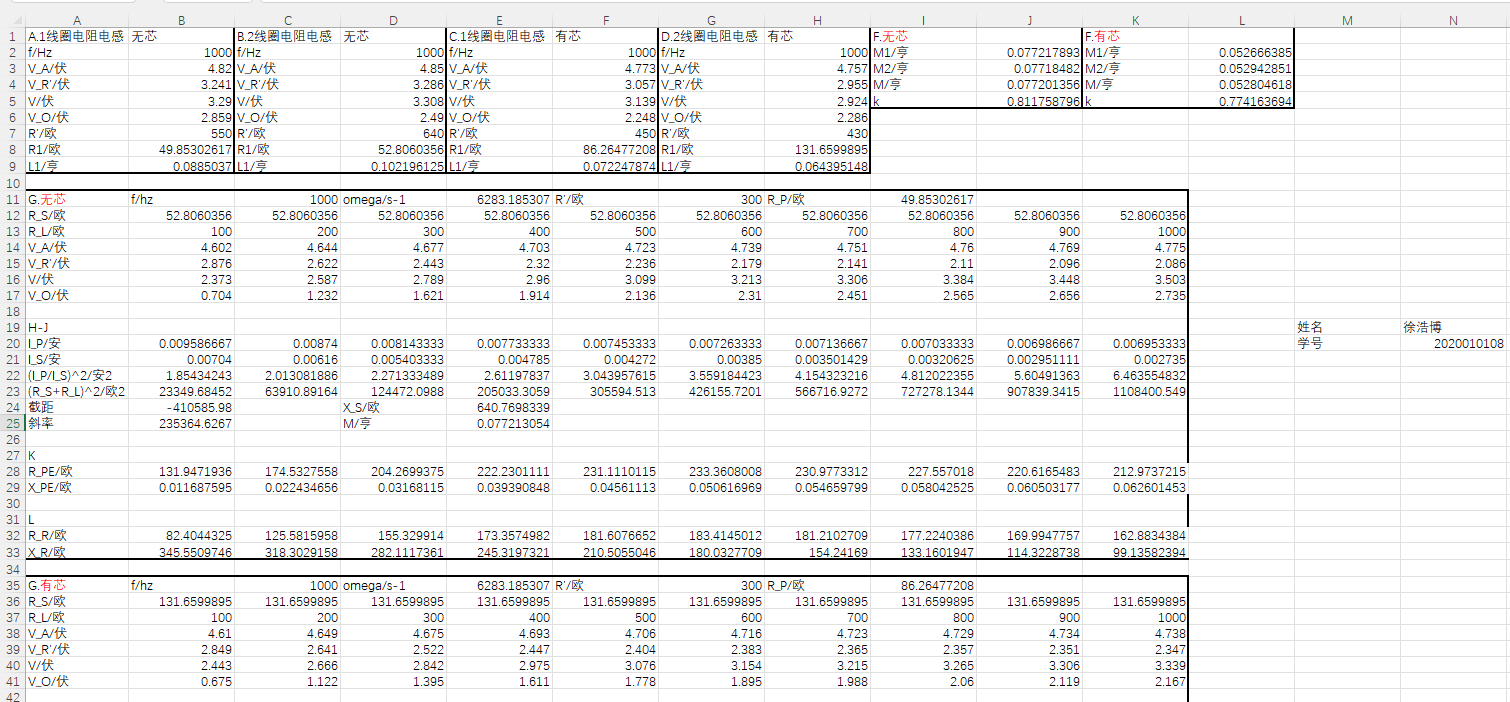
\includegraphics[scale=0.5]{data.PNG}
\end{center}\end{figure}

\end{document}

